\documentclass[a4paper,12pt]{article}
\usepackage[utf8]{inputenc}           % Codificação de entrada
\usepackage[T1]{fontenc}              % Codificação de fonte
\usepackage{lmodern}                  % Fonte moderna
\usepackage{xcolor}                   % Gerenciamento de cores
\usepackage{graphicx}                 % Inclusão de gráficos
\usepackage{hyperref}                 % Hyperlinks
\usepackage{amsmath}                  % Fórmulas matemáticas
\usepackage{geometry}                 % Configuração das margens
\usepackage{titling}                  % Customização de títulos
\usepackage{float}                    % Controle de posição de figuras
\usepackage{titlesec}                 % Customização dos títulos de seções
\usepackage{fancyhdr}                 % Cabeçalho e rodapé customizados
\usepackage[portuguese]{babel}        % Suporte ao português

% Configuração da geometria da página
\geometry{top=2cm, bottom=2cm, left=3cm, right=3cm}

% Configuração do hyperref
\hypersetup{
    colorlinks=true,
    linkcolor=blue,
    urlcolor=blue
}

% Configuração do cabeçalho e rodapé usando fancyhdr
\pagestyle{fancy}
\fancyhf{}
\fancyhead[L]{Universidade Tecnológica Federal do Paraná}
\fancyhead[R]{Oficina de Integração 1}
\fancyfoot[C]{\thepage}
\renewcommand{\headrulewidth}{0.4pt}
\renewcommand{\footrulewidth}{0.4pt}

% Customização dos títulos das seções com titlesec
\titleformat{\section}
  {\normalfont\Large\bfseries\color{}}{\thesection}{1em}{}
\titleformat{\subsection}
  {\normalfont\large\bfseries\color{}}{\thesubsection}{1em}{}

\date{\today}

\begin{document}

\vspace{1em}

\begin{center}
    \Large\textbf{Minichess com Machine Learning \\e Sistema CNC}
\end{center}

\vspace{1em}

% Autores e contatos
\begin{center}
    \textbf{Fernando Frare Vieira} \\
    \href{mailto:fernandofrarevieira@alunos.utfpr.edu.br}{fernandofrarevieira@alunos.utfpr.edu.br} \\
    +55 41 9900-6940 \\[1.5em]
    \textbf{Gabriel Affonso Borges Caballero} \\
    \href{mailto:gabrielaffonso@alunos.utfpr.edu.br}{gabrielaffonso@alunos.utfpr.edu.br} \\
    +55 41 9151-3335\\[1.5em]
    \textbf{Marco Vieira Busetti} \\
    \href{mailto:marcovieirabusetti@alunos.utfpr.edu.br}{marcovieirabusetti@alunos.utfpr.edu.br} \\
    +55 41 99798-4695
\end{center}

\vspace{1em}

\begin{center}
    \today
\end{center}

\vspace{2em}

\section{Introdução}
O projeto "Minichess com Machine Learning e Sistema CNC" \;foi desenvolvido com o propósito pedagógico de introduzir conceitos de Machine Learning para crianças. Utilizando um tabuleiro de xadrez simplificado (4x4), o sistema integra componentes de Inteligência Artificial e automação para demonstrar, de forma lúdica, como o aprendizado de máquina pode ser aplicado na prática. A solução proposta conta com um módulo de Visão Computacional, que realiza a captura do tabuleiro físico, e com um sistema CNC, que executa a movimentação automatizada das peças através da comunicação entre um computador e um Arduino.

\section{Motivação}
O principal objetivo deste projeto é educar crianças sobre os fundamentos do Machine Learning, uma área de extrema relevância na atualidade, por meio de uma experiência interativa e prática. Além disso, o Minichess 4x4 visa estimular o desenvolvimento do raciocínio lógico e da tomada de decisão, utilizando o xadrez simplificado como ferramenta de aprendizado. A integração dos componentes físicos (tabuleiro e sistema CNC) com a Inteligência Artificial oferece um ambiente dinâmico, onde o aluno interage diretamente com o jogo, consolidando os conceitos através da prática.

\section{Descrição Geral}
O Minichess 4x4 foi concebido para funcionar de forma integrada, utilizando um computador, uma câmera e um sistema CNC. Diferente de soluções que operam apenas por meio de interfaces gráficas, o jogo é realizado de modo físico: a criança posiciona as peças no tabuleiro real e o sistema, por meio da captura de imagem, interpreta a configuração atual e, em conjunto com a Inteligência Artificial, toma a decisão sobre o movimento. Posteriormente, o sistema CNC, controlado via comunicação serial com o Arduino, efetua a movimentação física das peças. Essa abordagem garante uma experiência completa e interativa, unindo teoria e prática. 

A integração é realizada através de APIs desenvolvidas em Python, utilizando o framework Flask para comunicação entre os módulos de Visão Computacional, Inteligência Artificial e controle CNC. O sistema CNC é baseado em um manipulador cartesiano com três graus de liberdade (eixos X, Y e Z), utilizando motores de passo Nema 17 em configuração CoreXY para movimentação precisa no plano horizontal, e um servo motor SG90 para controle vertical do eletroímã responsável pela movimentação das peças.

\begin{figure}[H]
    \centering
    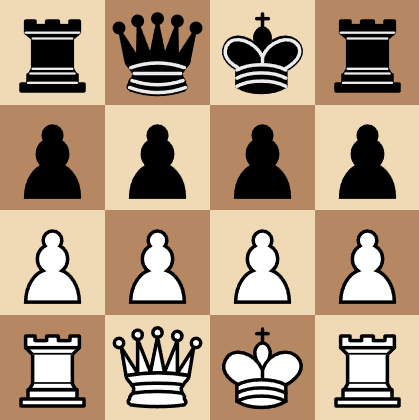
\includegraphics[width=0.5\textwidth]{images/minichess4x4.png} % Atualize com o caminho da imagem do modelo 3D ou do esquemático do CNC
    \caption{Tabuleiro do Minichess 4x4}
    \label{fig:modelo_cnc}
\end{figure}

\section{Diagrama de Blocos}
\begin{figure}[H]
    \centering
    \includegraphics[width=1.2\textwidth]{DiagramaMiniChess.drawio-3_page-0001} % Atualize o caminho para a imagem correspondente
    \caption{Diagrama de Blocos do Sistema Minichess}
    \label{fig:diagrama}
\end{figure}

\clearpage
\vspace{1em}

\section{Descrição do Software}
O software deste projeto é responsável por:
\begin{itemize}
    \item Implementar a lógica do jogo e a Inteligência Artificial com Machine Learning, utilizando o algoritmo \textbf{Q-learning} (aprendizado por reforço) para tomada de decisão. O agente aprende a otimizar suas jogadas através de um processo iterativo, onde cada ação é associada a um valor (\textbf{Q-value}) que representa a recompensa esperada em longo prazo. O algoritmo equilibra exploração (testar novas jogadas) e exploração (usar conhecimento adquirido), ajustando-se dinamicamente conforme interage com o jogador. A função de recompensa é definida para priorizar vitórias, evitar derrotas e incentivar movimentos estratégicos no tabuleiro 4x4.
    
    \item Capturar e processar imagens do tabuleiro físico utilizando a biblioteca OpenCV. As técnicas incluem detecção de cores (espaço HSV), filtragem de bordas (Canny) e comparação de contornos para identificar a posição das peças. A imagem é recortada para isolar o tabuleiro e evitar interferências externas.
    
    \item Gerenciar a comunicação entre o computador e o Arduino via protocolo serial, enviando comandos em G-Code para controle do sistema CNC. Uma API REST (desenvolvida com Flask) coordena o fluxo entre os subsistemas: após a jogada do usuário, a visão computacional envia o estado do tabuleiro para a IA, que retorna a ação aprendida pelo Q-learning, convertida em coordenadas para movimentação física pelo CNC.
\end{itemize}

\section{Descrição do Hardware}
Para a realização do jogo físico, o sistema conta com os seguintes componentes de hardware:
\begin{itemize}
    \item \textbf{Computador com Câmera:} Utilizado para capturar imagens do tabuleiro (resolução 1920x1080) e processar as informações necessárias para a tomada de decisão. A câmera é fixada em uma estrutura de suporte 3D impressa, posicionada verticalmente para garantir visibilidade total do tabuleiro.
    \item \textbf{Arduino UNO com CNC Shield V3:} Responsável por controlar os motores de passo (Nema 17) e o servo motor SG90. A CNC Shield utiliza drivers A4988 configurados em modo 1/4 de passo para equilibrar velocidade e precisão, e um relé JQC-3FF-S-Z para acionamento do eletroímã de 12V.
    \item \textbf{Sistema CNC CoreXY:} Composto por dois motores de passo para movimento no plano XY, seguindo o arranjo CoreXY para reduzir a inércia. O eixo Z é controlado por um servo motor, responsável por abaixar e levantar o eletroímã. A estrutura mecânica é baseada em perfis de MDF cortados a laser, com correias sincronizadas para transmissão de movimento.
    \item \textbf{Fonte de Alimentação:} Duas fontes de 12V 5A são utilizadas: uma para os motores de passo e ventoinhas de refrigeração, e outra exclusiva para o eletroímã.
\end{itemize}

\begin{figure}[H]
    \centering
    \includegraphics[width=0.5\textwidth]{images/modelo_CNC_page-0001} % Atualize com o caminho da imagem do modelo 3D ou do esquemático do CNC
    \caption{Referência do sistema CNC para movimentação física}
    \label{fig:modelo_cnc}
\end{figure}

\section{Lista de Componentes}
\begin{itemize}
    \item \textbf{Software:}
    \begin{itemize}
        \item Python 3.8+ (com bibliotecas OpenCV, Flask, NumPy, e PySerial)
        \item Firmware GRBL (para interpretação de G-Code no Arduino)
    \end{itemize}
    \item \textbf{Hardware:}
    \begin{itemize}
        \item Computador com câmera USB Full HD
        \item Arduino UNO + CNC Shield V3 + Drivers A4988
        \item 2x Motores de Passo Nema 17 + Correias GT2
        \item Servo Motor SG90 + Eletroímã 12V
        \item Fonte de Alimentação 12V 5A (2 unidades)
        \item Estrutura em MDF cortada a laser + Suportes 3D impressos
    \end{itemize}
\end{itemize}

\section{Integração entre Software e Hardware}
A comunicação entre os módulos é realizada através de APIs desenvolvidas em Flask, garantindo modularidade e escalabilidade. O fluxo segue três etapas:
\begin{enumerate}
    \item \textbf{Visão Computacional:} Após a jogada do usuário, a câmera captura uma imagem, processada pelo OpenCV para gerar uma matriz 4x4 representando o tabuleiro.
    \item \textbf{Inteligência Artificial:} A matriz é enviada para a API da IA, que executa o algoritmo de IA e retorna a coordenada jogada.
    \item \textbf{Controle CNC:} A coordenada é convertida em comandos G-Code (e.g., \texttt{G0 X10 Y5}) e enviada ao Arduino via serial. O CNC move o eletroímã até a peça, a transporta para a nova posição e retorna à origem.
\end{enumerate}

\vspace{1em}

\section{Cronograma}
\begin{figure}[H]
    \centering
    \includegraphics[width=1\textwidth]{images/ScreenshotCronograma1.png} % Atualize com o caminho da imagem do cronograma
    \caption{Diagrama de Gantt}
    \label{fig:cronograma_gantt}
\end{figure}

\vspace{1em}

\begin{figure}[H]
    \centering
    \includegraphics[width=1\textwidth]{images/Cronograma2.png} % Atualize com o caminho da segunda imagem do cronograma, se necessário
    \caption{Cronograma do Projeto}
    \label{fig:cronograma_projeto}
\end{figure}

\vspace{1em}

\begin{thebibliography}{9}
\bibitem{ref1} \href{https://arxiv.org/abs/2109.11434}{https://arxiv.org/abs/2109.11434}

\bibitem{ref2} \href{https://arxiv.org/abs/2106.11034}{https://arxiv.org/abs/2106.11034}

\bibitem{ref3} \href{https://journals.copmadrid.org/psed/art/psed2025a10}{https://journals.copmadrid.org/psed/art/psed2025a10}

\bibitem{ref4} \href{https://pubmed.ncbi.nlm.nih.gov/28494023/}{https://pubmed.ncbi.nlm.nih.gov/28494023/}

\bibitem{ref5} MakerC. \textit{DrawingBot: Open Source Plotter}. Thingiverse, 2016. Disponível em: \url{https://www.thingiverse.com/thing:2348062}.

\bibitem{ref6} Conrado, A. \textit{Controle de Máquinas CNC com GRBL}. Revista de Engenharia, 2017.

\bibitem{ref7} Handson Technology. \textit{CNC Shield V3 Documentation}. 2021. Disponível em: \url{https://www.handsontec.com}.

\end{thebibliography}

\end{document}
